% =====================================================================
% Sections IV-V. Companion to p3-intro-related-methodology.tex, whose
% roadmap paragraph promises these sections and which ends after Section III.
%
% Compiles on stock IEEEtran. No external image files: every figure is
% pgfplots with inline coordinates, generated by scripts/make_figures.py
% into docs/paper/figures/ and \input here.
%
% Requires, in the preamble:  \usepackage{pgfplots}\pgfplotsset{compat=1.18}
% =====================================================================

\section{Experimental Setup}
\label{sec:setup}

Section~\ref{sec:protocol} specifies the pre-registered protocol. This section
reports what has actually been executed against it, and says where the two
differ.

\subsection{What the pre-registered protocol requires, and its current status}

The kill-gate of Section~\ref{sec:protocol} is specified against the released
TTT-E2E checkpoint of Section~\ref{sec:sut} at 8K context, over five seeds per
condition. That configuration has not been run. Every gap between the harness and
a run on released weights is now closed: the experiment-tracking credential that
the reference implementation authenticates against before its evaluation branch
is reached is supplied, the requester-pays egress for the checkpoint and the
validation split is paid through a collaborator's account under their own
credentials, and the scale was brought down to hardware we already hold rather
than rented. Total expenditure on the project to date is \$0.13. What has not
happened is the run; no measurement in this paper was taken on released weights.

One departure from our own ordering has to be recorded here rather than left for
a reader to find. The per-update path of the gate --- the interceptor, the
anchor-consistency score, the update-uncertainty score and the decision policy
--- has been implemented, before the criterion of Section~\ref{sec:prereg}
returned a verdict, as a dated and signed revision to the pre-registration. The
protocol's own rule is that no demonstrated attack means no defense worth
building, and building the gate first inverts it. The reason was logistical: one
accelerator session can produce the attack verdict and a gate measurement
together, and sessions are the scarce resource. The cost is stated plainly. If the
criterion returns a stop, that work is sunk, and the claim that this project kept
the ordering is weakened to the narrower claim that it recorded the moment it
stopped keeping it. Two things were held fixed to limit the damage: no threshold
moved, and the design values inside the gate --- the symmetrized divergence, probe
rotation, scoring against $\anchorp$ --- remain pre-verdict choices labelled as
such rather than tuned findings, since the data that was to settle them does not
exist. The cumulative-drift path was not built at all, for the structural reason
given in Section~\ref{sec:driftstatus}.

What we report instead is a scaled-down pilot, and we are explicit that it
discharges nothing. Pre-registered thresholds are reported against, never moved.
The pilot renders no go/no-go verdict. Since it does not score the realism bar at
all, it cannot satisfy the conjunction in Table~\ref{tab:results} under any
circumstances; an unscored stream fails that bar safe, which is how a criterion
stated as a conjunction is meant to behave.

\subsection{The pilot configuration}

The pilot substitutes a byte-level model of roughly $10^5$ parameters,
implemented on the same JAX~\cite{bradbury2018jax} and
Equinox~\cite{kidger2021equinox} stack as the overlay of
Section~\ref{sec:interceptor}. Its frozen base weights are a token embedding, a
causal windowed-mean mixer and an output head. Its fast weights are a two-layer
position-wise MLP, zero-initialised into the residual stream. We train the base
weights \emph{through} the inner loop, taking the loss on each chunk after
adapting on its predecessors and differentiating that back into the slow weights,
which is what makes the fast weights load-bearing instead of decorative. At
inference, one inner SGD step is taken per 256-token chunk on that chunk's own
next-token cross-entropy, the same self-supervised objective the reference
implementation uses. Adapted weights carry across chunks through the overlay
described in Section~\ref{sec:interceptor}, exercised here through its
injected-seam interface without modification.

The corpus is 412\,KB of English prose, split into three disjoint slices: base
training, the attacker's source corpus, and a held-out evaluation slice. Benign
loss is always measured on the held-out slice, since measuring on the poison
stream itself is one of the invalidating conditions in Table~\ref{tab:prereg} of
Section~\ref{sec:protocol}. Each seed produces one poison stream and one control
stream that agree in length, chunk count, loss-bearing token count and precision,
and differ only in content.

We record two deviations from Section~\ref{sec:protocol} rather than absorbing
them. First, measurement freezes the fast weights instead of continuing to adapt
on the evaluation data. The protocol keeps adaptation on because freezing would
select a different code path in the reference implementation, a constraint the
pilot does not inherit, and freezing removes the decay confound. Second, the
inner learning rate is not supplied by a checkpoint and had to be chosen. We
selected the value that most improves held-out loss after adaptation \emph{on
benign text only}, before any poison stream existed, so that no part of the
poison-versus-control contrast enters the choice.

\subsection{Instrument validation}

The realism bar is a ratio of perplexities under a reference model, and that
model has to be independent of the victim. An attacker optimising against the
victim drives the victim's own perplexity down on exactly the streams the attack
shapes, so a bar scored with the victim would pass every attack by construction.

Two checks establish the instrument. One of them is a negative result, which we
report rather than discard. The acceptance check we originally specified was to
reproduce a published perplexity, and it turned out to be undecidable. The
published figure is per word, its word-count denominator is unspecified, and the
same measured total negative log-likelihood yields 62.29 under one convention and
31.18 under another, with the published 37.50 sitting between them. No outcome of
that check could separate an implementation fault from a counting convention, so
we record it as corroborating evidence and do not gate on it. What establishes
the implementation instead is logit-level equivalence against an independent
reference implementation: worst absolute logit difference $5.798\times10^{-4}$
against a $10^{-3}$ band, with argmax agreement 1.0000 at every sequence length
tested. A transposed weight layout, the wrong GELU variant, or a wrong
normalisation epsilon would each shift logits by $O(0.1)$, four orders of
magnitude outside that band.

Fig.~\ref{fig:fluency} reports the discrimination self-test and, in the same
panel, a limitation of one of our own pre-registered bars.

% Generated by scripts/make_figures.py.
% Source: experiments/001-attack-spike/FLUENCY_REFERENCE.md.
\begin{figure}[t]\centering
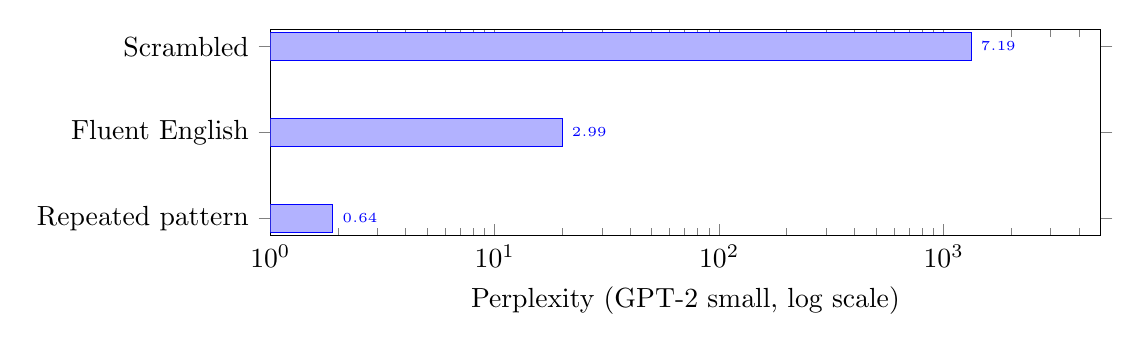
\begin{tikzpicture}
\begin{semilogxaxis}[width=\columnwidth,height=4.2cm,xbar,
  ytick={0,1,2},yticklabels={Repeated pattern,Fluent English,Scrambled},
  xlabel={Perplexity (GPT-2 small, log scale)},xmin=1,xmax=5000,
  nodes near coords,every node near coord/.append style={font=\tiny}]
\addplot coordinates {(1.90,0) (19.98,1) (1326.84,2)};
\end{semilogxaxis}
\end{tikzpicture}
\caption{Measured perplexity of three probe texts under the
independent reference model. The $66\times$ separation between fluent
and scrambled English is the discrimination self-test. The repeated
pattern at 1.90 is the negative result: perplexity rewards repetition,
so the $\rho \le 1.5$ realism bar cannot by itself reject a poison
stream that reuses one passage.}
\label{fig:fluency}
\end{figure}


Fluent English scores 19.98, and the same words scrambled score 1326.84, a
$66\times$ separation. A repeated short pattern, however, scores 1.90.
That is an order of magnitude better than real prose, because a repetitive stream
is trivially predictable. The realism bar therefore cannot reject a poison stream
that reuses one passage many times, though no human reader would call such a
stream benign-looking. We had flagged this on reasoning alone when span
granularity was decided; the measurement is what makes the two mitigations
already in place load-bearing rather than tidy. Spans are drawn without
replacement, and span multiplicity is reported per arm.

\subsection{Validity checks}
\label{sec:results}

Before reporting any effect, we have to know the inner loop is doing work. An
inert inner loop yields a null for reasons that have nothing to do with the
attack, and since the criterion is a stop rule, such a null is indistinguishable
from a real negative result. That is the most expensive failure available to this
experiment.

Our published structural check reads a falling per-token negative-log-likelihood
curve across one sequence, which detects a model adapting \emph{while} it reads.
It does not transfer to a pilot that freezes the fast weights during measurement,
so we ask the same question directly. Reading a benign document prefix moves the
loss on that document's own continuation from 2.5274 to 2.4592 nats/token, a gain
of 0.068 nats. The check passes, and the run aborts if it does not.

The noise floor was measured, not assumed. Two independent benign control streams
scored against each other give Cohen's $d = -0.557$ and a relative difference of
$-0.070\%$. This is what ordinary adaptation drift looks like here, and without it
no corruption number is interpretable.

\subsection{Headline result, and why its own negative control overturns it}

% Generated by scripts/make_figures.py -- do not edit by hand.
% Source: src/trustgate/eval/prereg.py (FROZEN), kept equal to
% experiments/001-attack-spike/PREREGISTERED.md by a CI test.
\begin{table}[t]
\caption{Pre-registered criteria, frozen 2026-07-28 before any attack code
was run. All four are required jointly. The observed column reports the
scaled-down pilot; it is \emph{not} the pre-registered verdict, which
requires the released 1B checkpoint and the GPT-2 fluency instrument.}
\label{tab:results}
\centering
\begin{tabular}{lcc}
\hline
Criterion & Pre-registered & Pilot (observed) \\
\hline
Effect size (Cohen's d), poison vs control & $\ge 0.80$ & 0.831 \\
Relative benign degradation & $\ge 10\%$ & +0.120\% \\
Fluency ratio vs control (max across seeds) & $\le 1.50$ & not scored (pilot) \\
Usable seeds per condition & $\ge 5$ & 5 \\
\hline
\end{tabular}
\end{table}

% Generated by scripts/make_figures.py.
\begin{figure}[t]\centering
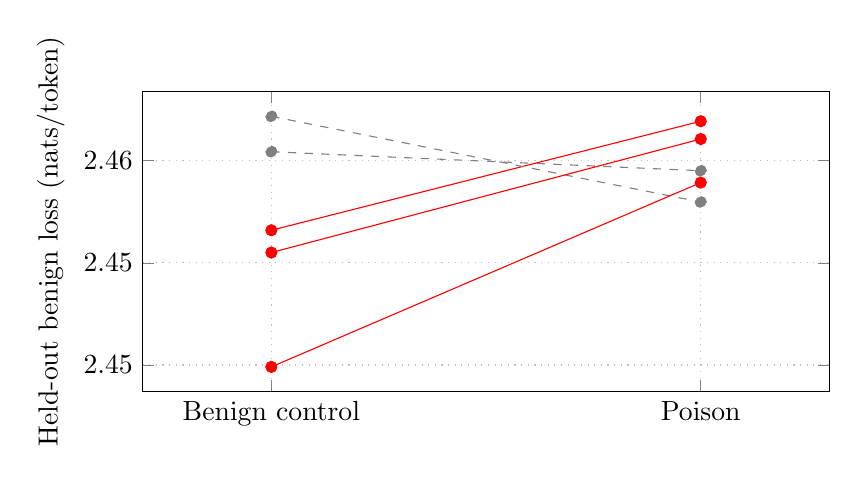
\begin{tikzpicture}
\begin{axis}[width=0.85\columnwidth,height=5.4cm,
  xtick={0,1},xticklabels={Benign control,Poison},
  xmin=-0.3,xmax=1.3,ylabel={Held-out benign loss (nats/token)},
  grid=both,grid style={dotted}]
\addplot[gray,dashed,mark=*] coordinates {(0,2.46043) (1,2.45950)};
\addplot[red,mark=*] coordinates {(0,2.45659) (1,2.46192)};
\addplot[gray,dashed,mark=*] coordinates {(0,2.46216) (1,2.45797)};
\addplot[red,mark=*] coordinates {(0,2.45550) (1,2.46105)};
\addplot[red,mark=*] coordinates {(0,2.44991) (1,2.45892)};
\end{axis}
\end{tikzpicture}
\caption{Per-seed benign loss after each stream, paired by seed. Dashed grey marks the seeds in which the poison stream helped the victim. Printing every seed is a standing requirement: an aggregate hides sign changes, and sign changes at this magnitude are better described as noise than as a weak attack.}
\label{fig:perseed}
\end{figure}


Table~\ref{tab:results} reports every pre-registered criterion beside the value
this pilot observed. Across five seeds the effect size, Cohen's $d$ with pooled
standard deviation~\cite{cohen1988}, is $d = 0.831$. That \emph{clears} the
pre-registered bar of 0.80. Relative degradation is $+0.120\%$ against a bar of
10\%, missing by roughly eightyfold. Read on its own, the first of those numbers
would look like a weak attack detected at the edge of the criterion.

It should not be read on its own. Fig.~\ref{fig:floor} puts it beside the
control-vs-control arm, in which two independent benign streams are scored
against each other and nothing is attacking anything.

% Generated alongside scripts/make_figures.py.
\begin{figure}[t]\centering
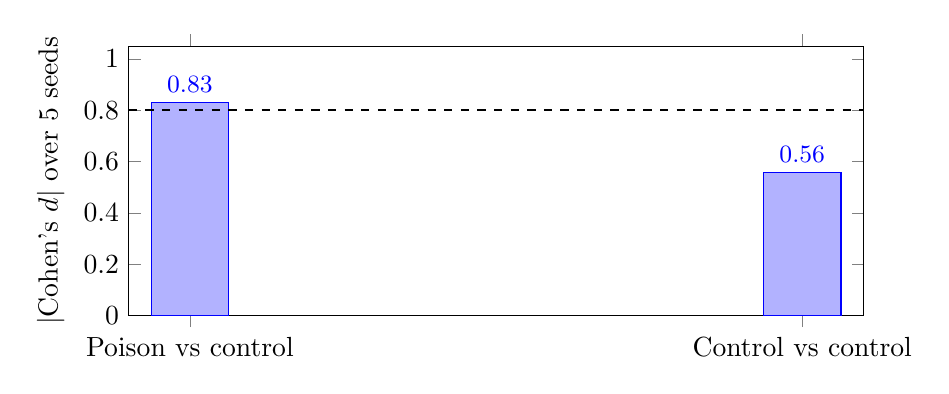
\begin{tikzpicture}
\begin{axis}[width=0.9\columnwidth,height=5cm,ybar,bar width=28pt,
  ytick={0,0.2,0.4,0.6,0.8,1.0},xtick={0,1},
  xticklabels={Poison vs control,Control vs control},
  ymin=0,ymax=1.05,ylabel={$|$Cohen's $d|$ over 5 seeds},
  nodes near coords,every node near coord/.append style={font=\small}]
\addplot coordinates {(0,0.831) (1,0.557)};
\draw[dashed,thick] ({rel axis cs:0,0}|-{axis cs:0,0.8}) -- ({rel axis cs:1,0}|-{axis cs:0,0.8});
\end{axis}
\end{tikzpicture}
\caption{The gating effect size beside its own negative control. The poison-vs-control measurement clears the pre-registered $d \geq 0.80$ bar (dashed), but the control-vs-control arm --- in which nothing is attacking anything --- reaches $|d| = 0.557$ on the same five seeds. A bar that a pure negative control can approach is not separating signal from noise at this sample size.}
\label{fig:floor}
\end{figure}


That negative control reaches $|d| = 0.557$ on the same five seeds. Our measured
``signal'' therefore sits within a factor of 1.5 of pure noise between two benign
streams. The honest reading is not that we found a weak attack. It is that
at five seeds the effect-size bar can be approached by noise alone, and
this run landed above it. Three further observations point the same way. Two of
the five seeds show the poison stream \emph{helping} the victim
(Fig.~\ref{fig:perseed}). The second statistical bar is missed by eightyfold, and
the two are pre-registered as a conjunction so that neither can carry a verdict
alone. The dose-response, below, is non-monotone and mostly negative.

This is what a negative control is for. Our protocol lists it as
reported-but-not-gating, justified as establishing that the corruption metric
measures corruption and not ordinary adaptation drift. Here it caught a false
positive that the gating statistic would have passed. We record two observations
about the instrument without acting on either, since pre-registered bars do not
move after a result is seen and a pilot is not the place to move one: $n=5$
appears under-powered for a $d \geq 0.8$ threshold, and an arm that can overturn
the gating statistic is doing more work than a non-gating label implies.

\subsection{The null distribution of the gating statistic}
\label{sec:null}

A single negative control shows that the bar \emph{can} be cleared without an
attacker. It does not say how often, and that difference matters: the first is an
anecdote, the second a false-positive rate. We therefore repeated the
control-vs-control arm twenty times on disjoint seed groups. Every draw compares
two benign streams over five seeds, so the true effect in every draw is exactly
zero by construction.

% Generated by experiments/002-pilot-tiny-ttt/run_null.py + make_figures.py.
\begin{figure}[t]\centering
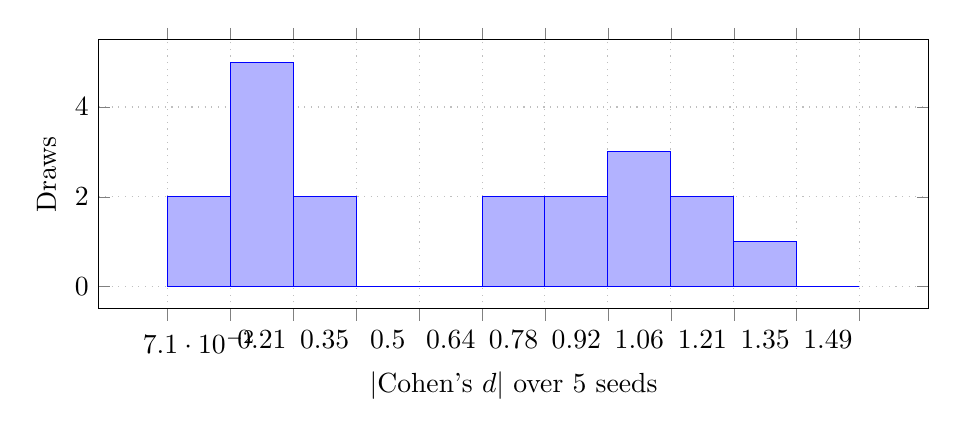
\begin{tikzpicture}
\begin{axis}[width=\columnwidth,height=5cm,ybar interval,
  xlabel={$|$Cohen's $d|$ over 5 seeds},ylabel={Draws},
  grid=both,grid style={dotted}]
\addplot coordinates {(0.071,2) (0.213,5) (0.354,2) (0.496,0) (0.638,0) (0.780,2) (0.921,2) (1.063,3) (1.205,2) (1.347,1) (1.488,0) (1.630,1)};
\end{axis}
\end{tikzpicture}
\caption{Null distribution of the gating effect size. Each of 20 draws compares two benign control streams over five seeds, so the true effect is zero by construction. Median $|d| = 0.816$; 11 of 20 draws clear the pre-registered $d \geq 0.80$ bar with no attacker present, a false-positive rate of 55\%. The deep run's observed $d = 0.831$ sits at the 55th percentile of this null.}
\label{fig:null}
\end{figure}


Fig.~\ref{fig:null} plots that null distribution with the observed value marked
on the same axis. Median $|d|$ under the null is 0.816; the mean is
0.695, the 90th percentile 1.227, the maximum 1.575. Eleven of twenty
draws, or 55\%, clear the pre-registered $d \geq 0.80$ bar with no attacker
present anywhere in the experiment. Our observed $d = 0.831$ sits at the
55th percentile of that null.

This settles how Section~\ref{sec:results} should be read. The headline effect
size is not a weak attack detected at the edge of a criterion. It is
approximately the median of what no attack at all produces at this sample size.
Reporting it as a positive result would have been a false positive, and the only
reason we did not is that the protocol required a negative control to be run and
reported whichever way it landed.

We draw two observations about the instrument and act on neither, since
pre-registered thresholds do not move once a result has been seen. First, five
seeds is under-powered for a $d \geq 0.8$ threshold in this configuration.
Second, an arm designated reported-but-not-gating has here overturned the gating
statistic, and would do so more often than not. Whether either observation
transfers to the released-checkpoint configuration of Section~\ref{sec:sut} is
unknown, because its noise floor has never
been measured. That is the point. This result is an argument for measuring the
noise floor \emph{before} the verdict is taken, not discovering it afterwards.

\subsection{Dose-response}

% Generated by scripts/make_figures.py.
\begin{figure}[t]\centering
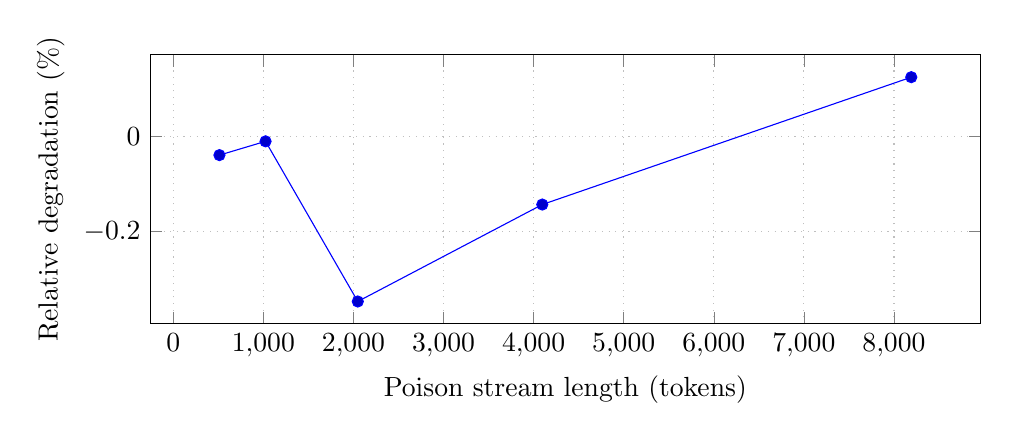
\begin{tikzpicture}
\begin{axis}[width=\columnwidth,height=5cm,
  xlabel={Poison stream length (tokens)},
  ylabel={Relative degradation (\%)},grid=both,grid style={dotted}]
\addplot coordinates {(512,-0.039) (1024,-0.010) (2048,-0.347) (4096,-0.143) (8192,0.125)};
\end{axis}
\end{tikzpicture}
\caption{Degradation against attack budget in the scaled-down
pilot. The pre-registration names stream tokens to threshold as a
secondary, non-gating metric.}
\label{fig:dose}
\end{figure}


Fig.~\ref{fig:dose} shows degradation against attack budget on two scales:
against the pre-registered bar, where the trend is invisible, and zoomed to the
data, where it can be read against the noise floor. The values are $-0.039\%$,
$-0.010\%$, $-0.347\%$, $-0.143\%$ and $+0.125\%$ at 512, 1024, 2048, 4096 and
8192 stream tokens. They are neither monotone nor consistently signed, and four
of the five favour the victim. An attack that accumulates with budget, which is
what the threat model describes and what the secondary ``slowness'' metric was
written to measure, does not look like this. The curve corroborates the reading
above: what the effect-size statistic picked up is seed noise, not a
dose-dependent effect.

Worth noting is that a shallower configuration, in which the base weights were
trained with the fast weights held fixed, produced a \emph{monotone}
dose-response of the opposite sign that rose with budget. That the trend
disappears once the base weights are meta-trained and the attacker is given a
search budget is itself informative. Apparent structure at this magnitude is not
stable across reasonable changes to the setup, which is the practical argument
for treating the noise floor as a required reading and not a courtesy.

\subsection{Discussion}
\label{sec:discussion}

\textit{What this result is evidence for, and what it is not.} It is evidence
that the pipeline is sound end to end: streams build, arms match, weights carry,
the metric computes, the report renders. It is also evidence that at this scale,
an attacker restricted to reordering real text spans does not measurably corrupt
fast weights. It is not evidence about TTT-E2E, and it is weaker evidence than
existing demonstrations of test-time poisoning against adaptation-based
systems~\cite{cong2024ttp,su2025realistic,hoang2024rip} would lead one to expect.
After meta-training, the pilot's inner loop is worth 0.068 nats within a
document, comfortably more than the 0.014 nats the mechanism under study buys at
8K, so the objection that there was too little adaptation to corrupt no longer
applies. What limits this run is statistical. At five seeds the gating effect
size is not separable from its own negative control.

\textit{The asymmetry the bar was set against.} Section~\ref{sec:prereg} states
it: ten per cent of a ${\sim}2.3$-nat baseline is roughly sixteen times what
test-time training buys at 8K. Nothing in this pilot changes that arithmetic, and
the scoping it implies applies here unchanged --- a null at this scale and this
context length is a null at this scale and this context length, not a claim that
fast weights are unpoisonable.

\textit{The weakest link is the attacker, not the defence.} Under the SELECT
strategy every span is real text and the only freedom is choice and ordering, a
deliberately weak lever chosen because a positive result under it would be
strong. Our pilot's ordering search is weaker still: hill-climbing over pairwise
swaps under a fixed evaluation budget, not the constrained search with the
realism term inside the objective that Section~\ref{sec:craft} specifies. A null
under a weak attacker is close to uninformative, and we prefer to say so.

\textit{A bar that cannot detect what it was written to detect.} The realism
constraint is a perplexity ratio, and perplexity rewards repetition
(Fig.~\ref{fig:fluency}). A stream that reuses one passage would pass the bar
while being obviously not benign-looking. This is why span multiplicity is
reported per arm, and it stayed at 1 in both arms here. The limitation belongs to
the pre-registered criterion, not to any particular result.

\section{Conclusion}
\label{sec:conclusion}

Fast weights as a short-term memory a network writes for
itself~\cite{ba2016fastweights}, and test-time training as adaptation to each
individual test input~\cite{sun2020ttt}, were until recently separate lines of
work. Their combination in modern long-context language
models~\cite{sun2024tttlayers,tandon2025tttE2E} carries a security consequence
the literature has not yet addressed: the serving path becomes a write path into
model state.

We have specified a threat model in which a benign-looking input stream steers a
test-time-training model's fast-weight updates so that later, unrelated benign
inputs are handled worse. We have specified a trust gate that intercepts each
proposed update against a frozen anchor, and proved a per-window drift bound for
the gated commit --- a bound that holds of the mechanism as specified and that our
own overlay does not yet enforce, for the structural reason recorded in
Section~\ref{sec:driftstatus}. And we have specified a criterion, frozen before
any attack code was written, that decides whether the defence is worth building at
all.

That criterion has not been discharged. A scaled-down pilot exercises the full
pipeline and returns an effect size that clears the bar, which its own negative
control then overturns: with no attacker present, the same statistic clears the
same bar on 55\% of draws, and our observed value sits at the median of that
null. We report no attack. What we contribute in its place is a measured
false-positive rate for a pre-registered criterion, together with the finding
that a negative control designated non-gating can overturn the gating statistic
more often than not at five seeds. The practical lesson is narrow and
transferable: a noise floor is not a courtesy reading taken after a verdict, it is
a precondition for the verdict having any content, and at five seeds a
conventional effect-size bar can be cleared by nothing at all.

We stated at the outset that no demonstrated attack means no defence worth
building, and the honest close is that we have not kept to it. The per-update path
of the gate was implemented before the criterion returned a verdict, recorded as a
dated revision rather than absorbed, and Section~\ref{sec:setup} states what that
costs if the verdict is a stop. The cumulative-drift path remains unbuilt, and is
the one component whose absence is structural rather than chosen. What survives
intact is the narrower discipline that produced the only result in this paper: the
bars did not move, the negative control was run and reported whichever way it
landed, and it was allowed to overturn the headline. That a protocol's own
reported-but-not-gating arm can invalidate its gating statistic is the finding we
would keep if we could keep only one.
